\documentclass[11pt]{article}
\usepackage[paper=a4paper, left=1cm, right=1cm, bottom=1.5cm, top=1.5cm]{geometry}

\usepackage{sectsty}
\usepackage{graphicx}
\usepackage{listings}

\begin{document}
\section{Base}

Es un arreglo de Bytes (8 Bits).
Cada Byte tiene una \textbf{unica} dirección.

\paragraph{Ejemplo}: Int es de 4 Bytes, entonces al crear un entero, C++
me reserva si o si 4 espacios de memoria contiguas.
En cambio al crear un Char, me guarda uno solo.
\vspace{.5cm}

No podemos decir a cual dirección quiero que se guarden las variables.
Pero si puedo saber en que dirección están.
De ahi la nocion de puntero.

El tipo T* es el tipo de los punteros a T.
Donde un puntero a T representa una direccion de memoria en la que
(presumiblemente) hay almacenado un valor de tipo T.

\paragraph{Ej:} int*: es un puntero a int.
int**: puntero a puntero.
\vspace{.5cm}

\paragraph{Forma de operar:}
\begin{itemize}
    \item Dirección de memoria de una variable. (\&\textbf{variable})
Si \textbf{variable} es de tipo T.
\&\textbf{variable} es de tipo T*.
Es decir me dice cual es la dirección que tiene esa variable.
Con esto básicamente me creo un puntero.
    \item Valor almacenado en una dirección de memoria. (operador de desreferencia)
        (*\textbf{puntero}).
Si \textbf{puntero} es de tipo T*.
*\textbf{puntero} es de tipo T.
Básicamente me dice el valor que tiene el lugar donde esta apuntando el puntero.
\end{itemize}

Si tengo un puntero, puedo en vez de usar el operador desreferencia, puedo usar
el operador  ''-$>$ ''.
Seria algo como, atraves del puntero p -$>$ x accedo a la variable que apunta.

\paragraph{Puntero nulo} = nullptr.
Puntero que no apunta a ninugn lado.
\subsection{Puntero}: Es una direccion de memoria representada por un entero en
hexagesimal y las podemos/debes conciderar como varibles.
Podemos pensar a la memoria como un arreglo unidimensional de Bytes.
Los tipos no importan para entender punteros.
Basicamente le decimos que tipo de datos suponemos que hay en esa direccion.
La idea es hacernos la vida facil pero mas alla de eso no importan.

Para \textbf{crear} un puntero lo hago con el tipo de elemento T y * (T* name).
El valor 0, NULL o nullptr, son todos analogos y son un puntero indefinido.
Para poder conocer la direccion donde esta alocada una variable lo hago con el simbolo
\& enfrente a dicha variable.
\begin{lstlisting}
    int var = 8;
    void* ptr = &var; \\ muestra que el tipo en realidad no importa
\end{lstlisting}

Si por ejemplo quiero declarar varios punteros en una misma linea,
tengo que agregar el simbolo para cada una de ellas.
Ej:\texttt{int* x, *y;}.
Para desferenciar un puntero hago lo mismo.
Agarro el puntero y adelante le pongo el simbolo *.
En nuestro caso, al decirle que es void tengo que decirle que tipo de dato
quiero almacenar ya que no lo sabe.
Si en cambio hago que ese puntero tenga el tipo int, al luego desferenciarlo y
le asigno un nuevo valor, este valor se va a tomar como un entero.

\begin{lstlisting}
    int var = 8;
    int* ptr = &var;
    *ptr = 10
\end{lstlisting}

Podemos hacer lo mismo en el \textit{heap}, agregando el caso de doble puntero.
\begin{lstlisting}
    char* bugger = new char[8];
    memset(buffer, 0, 8); \\ forma de asignar algo a un puntero. Valor 0 en 8
                          \\ posiciones.
    char** ptr = &buffer; \\Me da un puntero a la direccion donde esta
                          \\ guardado ese puntero.
   delete[] buffer;
\end{lstlisting}

\subsection{Referencia}:
Son casi iguales a los punteros.
Son una referencia a una variable.
No se puede inicializar una refernecia vacia y luego de inicializarla no la puedo
cambiar de referencia.
Y una referencia no es otra cosa que un alias, ya que la referencia no se guarda
en memoria, no es una copia ni nada.
Simplemente se hace una referencia al poner el tipo de variable T y \& (T\&).

Ejemplo un poco mas complicado:
\begin{lstlisting}
    void Increment(int* value){\\ El input es un puntero donde esta ese valor
        (*value)++; \\ lo desferencio y aumento el valor de esa variable.
    }

    int main(){
        int a =5;
        Increment(&a); \\ le estoy pasando la direccion en memoria
    }
\end{lstlisting}

No hay nada que se pueda hacer con referencias que no se puedan hacer con punteros.
Punteros son mas poderesos que las referencias, aunque este ultimo quizas hace
que el codigo sea mas limpio y facil de leer.

Diferencia:
\begin{lstlisting}
    int main(){
        int a = 5;
        int b = 8;
        \\ No se puede cambiar! Solo estoy haciendo que a = b = 8
        int& ref = a;
        ref = b;
        \\ Cambio el puntero que apunta a, al que apunta a b.
        int* ref = &a;
        *ref = 2; \\ a = 2
        ref = &b;
        *ref = 1; \\ b = 1
    }
\end{lstlisting}

\section{Clases}
Hay que pensarlas como que nos deja crear nuevos tipos de variables.
Las variables que estan definidas como clases, son las que se conocen como objetos.
Un nueva variable objeto se le llama instancia.
La diferencia para crear una clase es que despues del corchete va un semicomillas.

Dentro de la clase, todo es privado a menos que lo aclaremos.
Es decir solo las funciones de esa clase pueden acceder a las cosas de esa clase.
Las funciones que estan dentro de una clase se las denomina metodos.

La unica diferencia con los struct es que es todo publico por default.
Existe por compatibilidad por C.
En general se usa strcut para cosas sencillas y clases para cosas mas grandes.
Ejemplo si ya uso herencia, por convencion usamos clase.

\subsection{static}
Se distingue en dos tipos de uso, variables afuera de una clase o dentro.
Afuera de una funcion, lo que dice es que esa variable estatica solo se linkea al
momento de compilacion solo con las cosas de ese archivo.
Basicamente hace que esa variable no sea global para todos los archivos.
Esto es de ayuda ya que me evita tener el error de tener definido multiples veces
una variable con el mismo nombre.
Al hacerlo con \texttt{static} puedo declarar en otro archivo una variable
con el mimso nombre y el linker no las va a linkear.

Algo similar es el prefijo \texttt{extern}, que lo que hace es lo opuesto,
dice que esa variable viene de una variable definida en otro archivo, y entonces
al momento de la compilacion, va a buscar el linkeo.
Esto funciona siempre y cuando esa variable que voy a buscar no sea \texttt{static}.
Ya que ahi, es como que es ''privada'' para ese archivo donde se encuentra.

Con las funciones es exactamente lo mismo.
Dicho de otra forma, cuando uno declara una funcion o variable estatica,
solo va a ser visible dentro de ese archivo cpp donde se declaro.
En general es una buena constumbre usar esto para evitar que sean todas
funciones y variables globales a traves de todos los archivos cpp dentro de un
proyecto.

\paragraph{Dentro de una clase o struct}:
Lo que hace en este caso es hacer que esa funcion o variable no sean miembros de
la clase.
Hace que no haya instancias de estas variables, si no que se comparten con TODAS
las instancias.
Es como si fuera un namespace y no algo de una clase (aunque en realidad si lo
es ya que pueden ser publicas, privadas y demas).
Es decir, si cambio en una instancia una variable static, lo hace para TODAS
las demas instantaneamente.
Podemos pensarlo como si fueran punteros.
Ademas, estas variables hay que instanciarlas (no necesariamente inicializarlas)
dentro del codigo fuera de la clase.

\begin{lstlisting}
    struct Entity{
        static int x, y;
    }

    int Entity::x;

    int main(){
        Entity e;
        e.x = 1;

        Entity e1;
        e1.x = 3  \\ Cambio en TODAS x = 3, en la instancia e tambien;

        Entity::x = 2; \\ forma correcta, cambio a TODAS x=2
    }
\end{lstlisting}

Un metodo estatico, seria algo asi como si en python un metodo no
tuviera implicito el self.
Esto hace que no tenga una instancia, es decir no puede acceder a variables que son
de UNA instancia en particular.

\paragraph{Local static}
Dentro de una funcion, si hago una variable estatica, es como si en realidad la
estuviera incicializando afuera.
Es decir si hago \texttt{static int i = 0;} dentro de una funcion, y dentro de ahi
le agrego 1.
Cada vez que la llame va a recordar que valor tiene, e ira sumando 1.
Si no estuviera el static, lo que haria seria siempre definirla como 0, y agregarle
1, devolviendo siempre 1.
Es como que se define una unica vez.
Lo que tiene de bueno a diferencia de definirla afuera, es que de esta manera
el scope de esta variable es local a la funcion, y no me permite modificarla
desde afuera.

\subsection{Enumns}
Algo cortito, muchas veces queremos definir una palabra o algo igual a un numero.
Existe enum, que hace esto.
Puede meterse dentro de una clase o lo que sea.
Ademas puedo decir que tipo son los enum, por default es int.
\begin{lstlisting}
    class Log{
        public:
        enum Level:{  \\ por default arranca en cero y podria no aclararlo
                  \\ tambien va sumando de a 1, asi que podria asignar uno solo y
                  \\ el resto se va a acomodar
        Error=0, Warning=1, Info \\ va a ser 2 este ultimo
        }
        vodi SetLevel(Level level){
            m_LogLevel = level;
        }
        private:
        Level m_LogLevel = Info;
    }
    int main(){
        Log log;
        log.SetLevel(Log::Error);
    }
\end{lstlisting}


Existe la clase enum la cual nos permite definir namespace.
\subsection{Const}
El const hay que pensarla como una promesa.
Que prometemos hacer algo constante, aunque facilmente podemos romper esa promesa.

Casos en variables:
\begin{itemize}
    \item const type* a =...: Aca el const dice que donde apunta el puntero es constante
            y no el puntero en si. Puedo cambiar a que apunte a otro lado.
    \item type const* a=...: Exactamente igual al caso anterior.
    \item type* const a =...: Aca estoy diciendo que es constante el puntero, pero si
        puedo modificar lo que esta en la  direccion que apunta.
    \item const type* const a =...: La combinacion de ambos casos.
\end{itemize}

El const tambien se usa en el contexto de clases.
Por ejemplo si en un metodo le agregamos al final const, lo que dice es que ese
metodo no va a poder cambiar ninguna variable de la clase, basicamente va a ser
un metodo de lectura solo, por ejemplo un getter.

Queda el por que ponerlo como const.
En la mayoria de casos, uno quiere usar funciones que su input sea por referencia
ya que no quiero estar copiando siempre.
Entonces en general puedo pasar una referencia constante a una funcion.
Si esa funcion que recibe un input de clase constante quiere usar un metodo
que puede cambiar ese input no se va a poder.
Es por esto que ese metodo tiene que tambien ser constante, para asegurar
que no se va a modificar ese input.
Puedo tener exactamente dos metodos una con const y otra sin, y C++
se va a encargar de usarlas convenientemente.

Ej:
\begin{lstlisting}
    class Entity{
        private:
            int m_X, m_Y;
        pulbic:
            int GetX() const{
                return m_X;
            }
    }

    void PrintEntity(const Entity& e){
        std::cout << e.GetX() << std::endl;
    }

    int main(){
        Entity e;
    }
\end{lstlisting}

Hay algo en C++ que se llama mutable, que lo que hace es ponerse al principio de
la declaracion de una variable (va antes del tipo) y lo que hace es que ESA variable
pueda ser modificada aun en un metodo con const.


%%%%%%%%%%%%%%%%%%%%%%%%%%%%%%%%%%%%%%%%%%%%%%%%%%%%%%%%%%%%%%%%%%%%%%%%

%%%%%%%%%%%%%%%%%%%%%%%%%%%%%%%%%%%%%%%%%%%%%%%%%%%%%%%%%%%%%%%%%%%%%%%%

\section{Modelo de Memoria C++}


\subsection{Regiones de memoria}
Un programa en C/C++ almacena sus datos en memoria en tres áreas diferentes:
Estas estan en la RAM.
En general nos vamos a concentrar en la diferencia entre el \texttt{Stack} y el \texttt{Heap}
En el inicio del programa estas dos secciones de memoria ya estan asignadas y
separadas (algo asi... dar mas info).
\begin{enumerate}
    \item Memoria global.
        Es el área en la que están almacenadas las variables
        que se declaran globales o estáticas y las constantes de tipo cadena de caracteres (por ejemplo "Mi string").
        Es decir, en esta zona de memoria se almacenan todos aquellos datos que
        están presentes desde el comienzo del programa hasta que termina.
    \item Stack o La pila (se administra automaticamente).
        Es un área en la que las variables aparecen y desaparecen en un momento
        puntual de la ejecución de un programa.
        El tiempo de vida de una varialbe esta dado por su scope.
        Se utiliza principalmente para almacenar variables locales a las funciones.
        Estas variables tienen un ámbito reducido, sólo están disponibles mientras
        se está ejecutando la función en la que han sido definidas.
        En la pila se encuentran todas estas variables, y por tanto, en esa zona
        se está continuamente insertando y borrando variables nuevas.
        Si una funcion f llama a otra g. Esta ultima puede usar todavia las variables de
        f, ya que el scope de f todavia no termino.
    \item El heap (se administra manualmente).
        Esta zona (traducida en algunos casos como “el montón”) contiene memoria
        disponible para que se reserve y libere en cualquier momento durante la
        ejecución de un programa.
        No está dedicada a variables locales de las funciones como la pila, sino
        que es memoria denominada “dinámica” para estructuras de datos que no se
        saben si se necesitan, e incluso tampoco se sabe su tamaño hasta que el
        programa está ejecutando.
\end{enumerate}

El heap tiene dos operaciones para administrar la memoria dinamica.
\begin{itemize}
    \item new T: Reserva espacio en el heap para almacenar un valor
        de tipo T. Devuelve un puntero de tipo T* a la direccion de memoria
        donde comienza ese espacio.
    \item delete p: libera la memoria asociada al puntero p.
        Si borro todos los punteros que apuntan a esa direccion pierden la posibilidad
        de acceder a ella.
\end{itemize}

Existen estas dos operaciones con corchetes, generando espacio contiguo en memoria heap.
new T[n]:Devuelve un puntero de tipo T* a la direccion de memoria donde comienza ese espacio.
delete[] p: libera la memoria asociada al arreglo que empeiza en la  direccion p.

Ej de hacer lo mismo con stack vs heap:
\begin{lstlisting}
    strcut Vector3{
        float x, y, z;

        Vector3(): x(10), y(11), z(12){}
    }
    int main(){
        int stack_value = 5;
        int stack_array[5];
        stack_array[0] = 1; \\ puedo inicializar cualquiera de ellos
        Vector3 stack_vector;

        int* heap_value = new int;
        *heap_value = 5;
        int* heap_array = new int[5];
        heap_array[0] = 1;
        Vector3* heap_vector = new Vector3();

        delete heap_value;
        delete[] heap_array;
        delete  heap_vector;
    }
\end{lstlisting}

El stack, solo mueve el puntero del stack una cierta cantidad de memoria y
asigna ahi.
Es una pila de data, que vamos apilando a medida que voy pidiendo.
Si quiero agregar un int, solo muevo 4 lugares el puntero eso y ahi meto el int.
Es decir me da esa direccion de memoria.
Es muy rapido el stack ya que es basicamente una unica instruccion de CPU.
El tema es que esta memoria se guarda solo durante la duracion del scope que se
encuentre.
Despues de ahi automaticamente se borra, algo que muchas veces queremos
pero otras no.

El heap es distinto, no estan estan de forma ordenada ni se borran de forma
automatica.
Un array obviamente si esta ordenado, ya que se pidio de una vez ese espacio en memoria.



\paragraph{Problemas}
\begin{enumerate}
    \item leak: Reservar espacio del heap y no liberarlo al dejar de usarlo.
    \item dangling pointers: Luego de hacer delete de una direccion de memoria, tener
        punteros que siguen apuntando ahi.
    \item Doble delete.
    \item Desfrefrencia de NULL (*NULL).
\end{enumerate}

\subsection{Destructor}
Para solucionar los leaks se crean los destructores.
Cada vez que se libera la memoria de un objeto del tipo T, C++ invoca implicitamente
al \textbf{destructor} del tipo T.
El destructor de una clase T se llama T::~T(), el cual esta en public de la clase.
El programador nunca debe llamar explicitameante al destructor.

\subsection{Referencias}
Una variable local o parametro se puede declarar como una referencia a un valor de
tipo T, dandole tipo T\&.
Las referencias son punteros que no puede cambiar el lugar al que apunta
durante su ciclo de vida.

Ejemplo:
\begin{figure}[h]
    \centering
    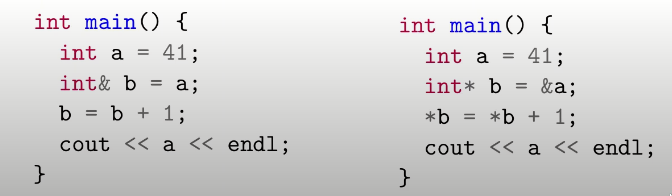
\includegraphics[width=0.9\textwidth]{referencia.png}
    \caption{Referencia vs puntero  haciendo lo mismo.}
    \label{fig:ref}
\end{figure}

Si tengo dos variables int, $x$ e $y$ y digo que una referencia r sea igual a x.
Luego si digo que r sea igual a y, lo que sucede no es que ahora r es referencia de
y, si no que a x le asigna el valor de y. Ya que r es una referencia de x para el
largo de su ciclo de vida.

\paragraph{Devolucion de reusultados por referencia}.
El mejor ejemplo es el operador [], el cual esta dandole una referencia
del espacio en memoria de ese lugar del arreglo.
\vspace{0.5cm}

Para funciones, existe el pasar por referencia constante (const T\&).
El cual tiene el beneficio de no tener que hacer una copia del input, si no simplemente
poder acceder a ella, pero con la seguridad de que no nos va a permitir modificarla.
Ejemplo una funcion que dado un vector nos devuelve el valor de la suma de sus dos primeros
elementos.
Si le paso un vector gigante, es ultra ineficiente tener que hacer una copia de un
vector gigante solo para devolver la suma de sus dos primeros elementos...
Y pasarlo por referencia puede ser inseguro ya que nada nos asegura que esa funcion
internamente no nos modifique al vector.
Por eso existe por referencia constante.

\section{Constructores}
Cuando yo desclaro una clase en mi codigo, automaticamente se me reserva en la pila
memoria para todas las variables que estan declaradas de forma privada dentro de
la clase.
Si no tengo un constructor, esos valores quedan indefinidos (basura).

Ej: \ref{fig:const}.
\begin{figure}[h!]
    \centering
    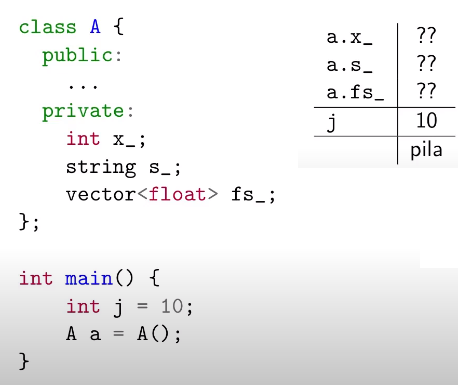
\includegraphics[width=0.7\textwidth]{constructor.png}
    \caption{Ejemplo de la reserva de memoria al declarar una clase.}
    \label{fig:const}
\end{figure}

Las consideraciones especiales del constructor.
\begin{itemize}
    \item Se escriben con el nombre del tipo.
    \item no tienen tipo de retorno (esta implicito).
    \item Tres formas de constructores:(Ej, clase Horario)
        \begin{itemize}
            \item Por defecto: Horario();
            \item Por copia: Horario(const Horario\&);
            \item Con parametro: Horario(int hora,...);
        \end{itemize}
    \item Cuando defino un constructor desaparece el cosntructor sin parametros
            implicito.
\end{itemize}

\subsection{Struct y member class}
Los struct son iguales que las clases, con la diferencia que las cosas que escribo
dentro de strcut son publicas.
En las clases por defecto son privadas.
El uso que se le suele dar es para estructuras de datos sencillas, cuando no
necesitamos un modulo armado al 100\%.
En general para cosas mas chiquitas y en general todo publico.
Un uso comun es para armarme tuplas donde le pongo nombre a cada elemento.

Otro uso importante, es usar a struct dentro de una clase.
Por ejemplo en una clase Lista, puedo armar un struct Nodo adentro.
Podria armar un struct Nodo afuera, pero si ademas quiero un struct Nodo
para otra clase, ej conjunto, la cual tendra diferentes cosas, empeizan a pisarse
y necesitaria armar con diferente nombre dos struct Nodos.
Como en ambos casos el struct Nodo tiene sentido solo en contexto de cada clase,
armo el struct dentro de ese contexto/clase.
Un ejemplo puede verse en \ref{fig:nodo}.

\begin{figure}[h!]
    \centering
    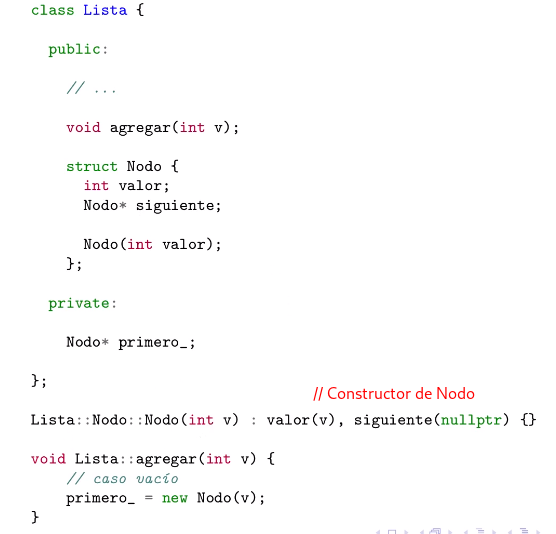
\includegraphics[width=0.7\textwidth]{nodo.png}
    \caption{Ejemplo de struct dentro de clase, y el contructor de nodo.}
    \label{fig:nodo}
\end{figure}


En general, en estos casos, tambien se aclara que ese struct es privado dentro
de la clase.
La clase no tiene por si misma las cosas de la struct.

\vspace{0.5cm}
\paragraph{friend}: Se le dice a la clase, que funciones (o quizas algo mas, chequear),
tiene  acceso a la parte privada de su clase.
Esto se declara en public, ''friend int main();''.
Donde ahi dice que desde la funcion main() se puede acceder a la parte privada,
pudiendo asi hacer ''List::Nodo n(5);''.
Donde recordemos que la struct nodo esta en la parte privada.
Otro uso es hacer friend a los operadores externos como, ''='', ''$<<$'', etc.
\end{document}

